\subsection{\label{subsec:FZV2}Frage 2}
\textbf{\textit{Wie sehen die Feld- und Ladungsträgerverteilung der plasmonischen Grundmode aus?}}\\
$\rightarrow$Zunächst schränken wir uns auf die Betrachtung eines lokalisierten Partikelplasmons 
ein, um die Beschreibung für Volumen- oder nicht lokalisierte Oberflächenplasmonen zu umgehen.
Vereinfacht ausgedrückt entsteht das Partikelplasmon durch die Wechselwirkung der freien Elektronen 
im Leitungsband eines Partikels mit einem elektrischen Feld \cite{Anleitung}. 
Dies führt zu einer Ladungstrennung und durch die resultierende Coulomb-(Rückstell-)Kraft zu einer Schwingung, 
wobei die Grundmode das Dipol-Partikelplasmon ist \cite{FZV2p3}. 
Die Effizienz der Modenanregung hängt von der Lichtfrequenz und der Polarisation ab, wobei 
Frequenz des Lichtes im Bereich der Eigenfrequenz der betrachteten Mode liegen sollte und 
die Polarisation in Schwingungsrichtung der Mode gewählt werden sollte. 
Die genaue Ladungsverteilung und das elektrische Feld sind von der Form des Nanopartikels abhängig, 
was gezielte Anwendungen durch das Design unterschiedlicher Formen ermöglicht \cite{FZV2p1}. 
Für die ersten beiden Moden ist das elektrische Feld und die grobe Ladungsverteilung 
in Abb.~\ref{fig:moden} skizziert.
\begin{figure}[h!]
    \centering
    \subfloat[\centering Dipol]{{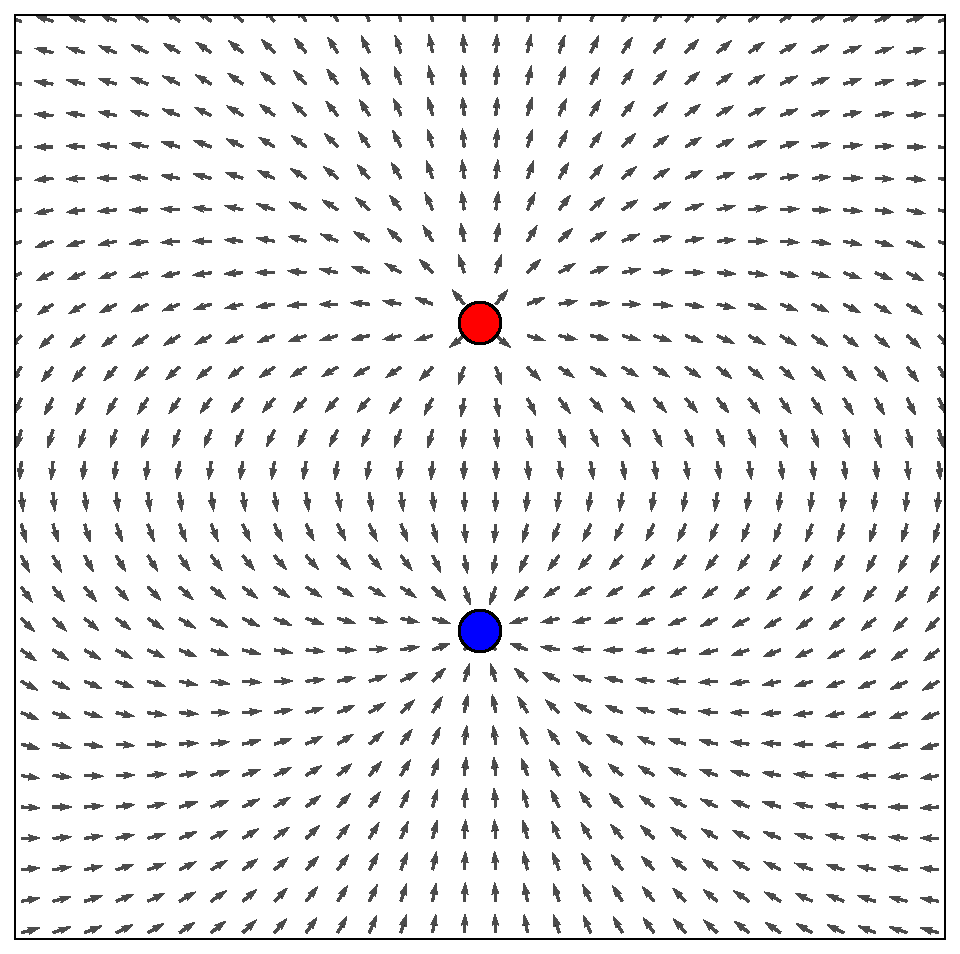
\includegraphics[width=0.45\textwidth]{c1.pdf} }}
    \qquad
    \subfloat[\centering Quadrupol]{{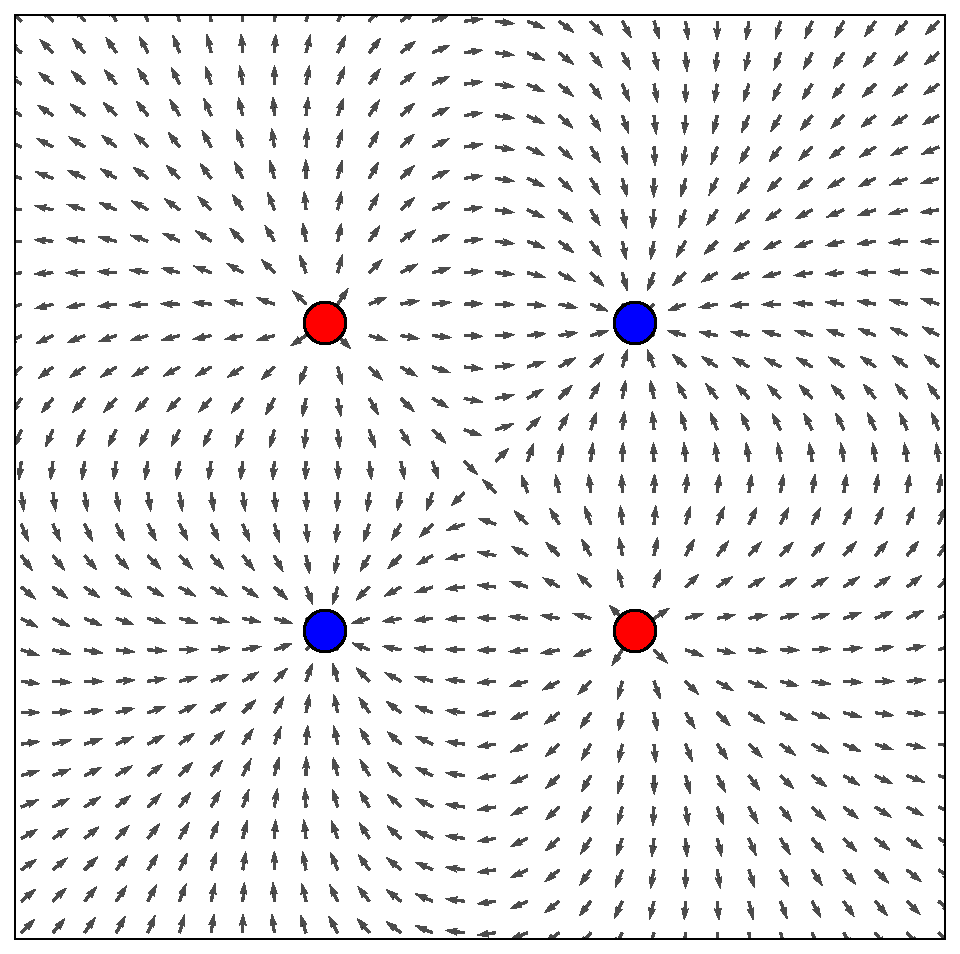
\includegraphics[width=0.45\textwidth]{c2.pdf} }}
    \caption{\label{fig:moden}Skizze des elektrischen Feldes (schwarze Pfeile) eines 
    Dipols und eines Quadrupols, 
    sowie die jeweiligen Ladungen (rot=positiv, blau=negativ).
    Eine elektromagnetische Welle kann zu einer lokalen Ladungstrennung innerhalb des
    Nanopartikels führen, die ein E-Feld erzeugt. Das tatsächliche Feld 
    hängt von der Form des Nanopartikels ab und ist hier daher sehr allgemein gehalten.}
\end{figure}\FloatBarrier \,\\

\textbf{\textit{Beschreiben Sie, warum es Plasmon-Moden gibt, die unter einem Mikroskop
mit Laserlicht nicht angeregt werden können. Skizzieren Sie auch hier die Feld- und
Ladungsträgerverteilung einer solchen Mode. Wie kann man solch eine Mode dennoch anregen?}}\\
$\rightarrow$Die nächst höhere Mode, das Quadrupol-Partikelplasmon, 
zeigt eine weiter verfeinerte lokale Ladungstrennung. Die Anregung durch Laserlicht kann erschwert werden, 
da sich die Schwingungsrichtung im Vergleich zur Dipol-Mode dreht und die Eigenfrequenz der Mode verändert 
ist. Zudem muss im Allgemeinen darauf geachtet werden, dass das anzuregende Plasmon die gleiche 
Schwingungsrichtung (gekoppelt mit der Ausbreitungsrichtung) wie das anregende Licht hat.
Longitudinale Oberflächenplasmonen können beispielsweise nicht von transversalen Lichtwellen 
angeregt werden \cite{FZV2p2}. \\
Weitere Multipol-Partikelplasmonen können durch geeignete Formen, Einstrahlwinkel, Polarisation 
und Lichtfrequenz angeregt werden. 
Im Gegensatz zu schmalbandigem Laserlicht ermöglicht die Bestrahlung mit weißem 
Licht eine breitere Modenanregung. 